\setchapterpreamble[u]{%
    \margintoc\hfil
    \dictum[Richard Feynman]{What I cannot create,\\I do not understand.}
}

\chapter{Methods}
\labch{methods}
% Write in theorem-proof fashion

The following sections describe the design and build process --- including the reasoning behind the decisions taken --- of the \magnethical{} NMR spectrometer. \reffig{block-diagram} shows an overview schematic of the main components that will be discussed.

\begin{figure}[hbt]
    \centering
    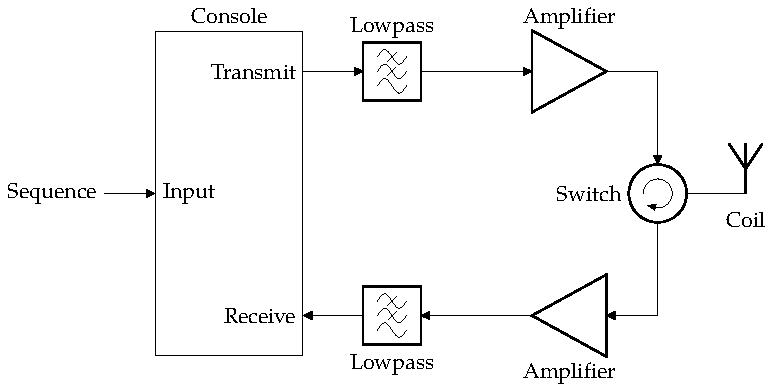
\includegraphics{images/block_diagram.pdf}
    \caption{\captiontitle{Block Diagram.} The main components of the \magnethical{} NMR spectrometer, including the console, lowpass filters, analogue amplifiers, transmit-receive switch and transmit-receive coil.}
    \labfig{block-diagram}
\end{figure}

The section order follows the path of the signal, that is, clockwise around the schematic starting with the console.

\section{The console}
\begin{marginfigure}[-4.5\baselineskip]
    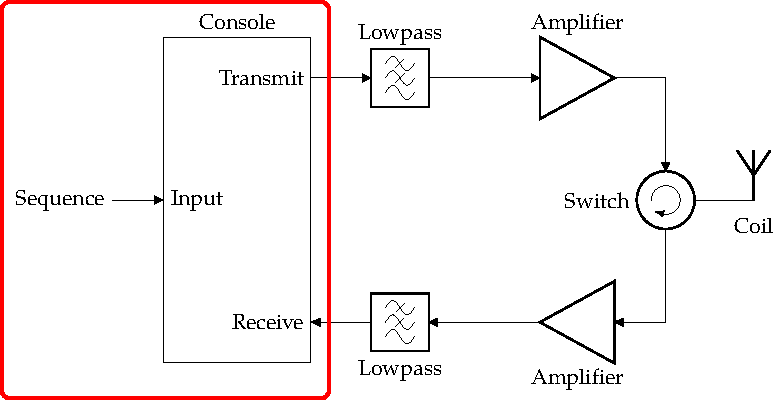
\includegraphics{block_diagram_highlight_console.pdf}
    \labfig{block-diagram-console}
\end{marginfigure}

The relatively low frequency of \(f_0 = \qty{25}{\mega\hertz}\)\sidenote{Given by the \ch{^1H} resonance frequency in the \qty{0.6}{\tesla} magnet} as well as the low bandwidth of only about \qty{10}{ppm}\sidenote{Equals \qty{25}{\hertz} at \qty{25}{\mega\hertz}} of the expected signal allows moving a lot of previously analogue tasks into the digital domain, greatly simplifying the hardware setup and making it more flexible. According to the Nyquist theorem, the minimum frequency that can be used to digitize an analogue signal without loss of information\sidenote{That is, without aliasing issues} must be more than twice as large as the highest frequency component of interest in the signal. In our case, the analogue-to-digital conversion must happen with more than
\[
    f_{min} \ge 2f_0 = \qty{50}{\mega\hertz}
\]
if oversampling is to be used. The setup could also make use of the low bandwidth of the signal and use the aliasing effect of the analogue-to-digital conversion to its advantage using undersampling. Since this requires taking further care when sampling and filtering, and the expected frequencies are low enough to make oversampling feasible, oversampling is employed in this setup. This has the added advantage of higher flexibility since the sampling frequency can be easily adjusted downwards.

For digital processing, a \acrfull{fpga} is used, which can be thought of as a piece of programmable hardware. To ease development a ready-made \acrshort{fpga} board --- the RedPitaya SDRlab 122-16 --- was chosen. With a sampling frequency of \qty{122.88}{\mega\sample\per\second} it is well above the Nyquist limit. Combined with a resolution of \qty{16}{bit} it is more than capable of capturing all relevant data from the analogue signal. Due to the commercial nature, the board is easily procured directly from RedPitaya or any of the well-known distributors\sidenote{For example Digikey, Mouser, Farnell, \dots}. A possible open-source alternative in the future would be the LimeSDR\sidenote{\url{https://limemicro.com/products/boards/limesdr/}}. With a sampling frequency of \qty{61.44}{\mega\sample\per\second}, limited by the USB3 interface, and a resolution of \qty{12}{bit} it is less powerful than the RedPitaya, but still fast enough for oversampling without loss of information. This board would cost less than half (\approx 280CHF) of the RedPitaya board and would enable a completely open design of the spectrometer --- in line with the accessibility goals of this work. Unfortunately, due to the young age of this project and the crowd-sourced nature, no board was available for purchase at the time of writing.

After sampling the signal is demodulated using a quadrature detection system by multiplying it with the signal of a complex numerically controlled local oscillator. The same principle is applied inversely on the sending side for modulation. The resulting complex demodulated signal is then passed through a \acrfull{cic} filter for low-pass filtering and decimation to filter out high-frequency components of the signal and reduce the size of the data stream. The full data steam would incur a bandwidth of
\[
    \qty{16}{\bit} \cdot \qty{122.88}{\mega\sample\per\second} = \qty{245.76}{\mega\byte\per\second}
\]
per channel. With potentially 2 transmit and 2 receive channels this results in a data rate of close to \qty{1}{\giga\byte\per\second}, which is way higher than the theoretical limit of \qty{116}{\mega\byte\per\second} of the Ethernet interface. Due to inefficiencies in the Linux kernel of the RedPitaya Image, the practical data rate limit for continuous streaming is a lot lower at about \qty{20}{\mega\sample\per\second}\sidenote{According to the official \gls{lcrmeter} documentation (\url{https://redpitaya.readthedocs.io/en/latest/appsFeatures/applications/streaming/appStreaming.html})}. This has been improved in Pavel Demin's kernel image, where speeds up to \qty{80}{\mega\byte\per\second} have been measured\sidenote{\url{https://pavel-demin.github.io/red-pitaya-notes/alpine/}}. However, this only becomes relevant on long acquisition times over several seconds and hasn't been thoroughly tested as it hasn't been relevant, yet.

All of these digital signal-processing tasks are performed by the \acrshort{marcos} \acrshort{fpga} firmware developed by Vlad Negnevitsky\sidecite{negnevitskyMaRCoSOpensourceElectronic2023}. The system is designed for a low-field MRI system but could be easily adapted for NMR spectroscopy. The demodulated, filtered and decimated data from MaRCoS is then sent through its C server to the developed high-level Python interface. \reffig{marcos} shows an overview of the \acrshort{marcos} architecture. For more information on the Python programming interface see \refsec{software}.

\begin{figure}[hbt]
    \centering
    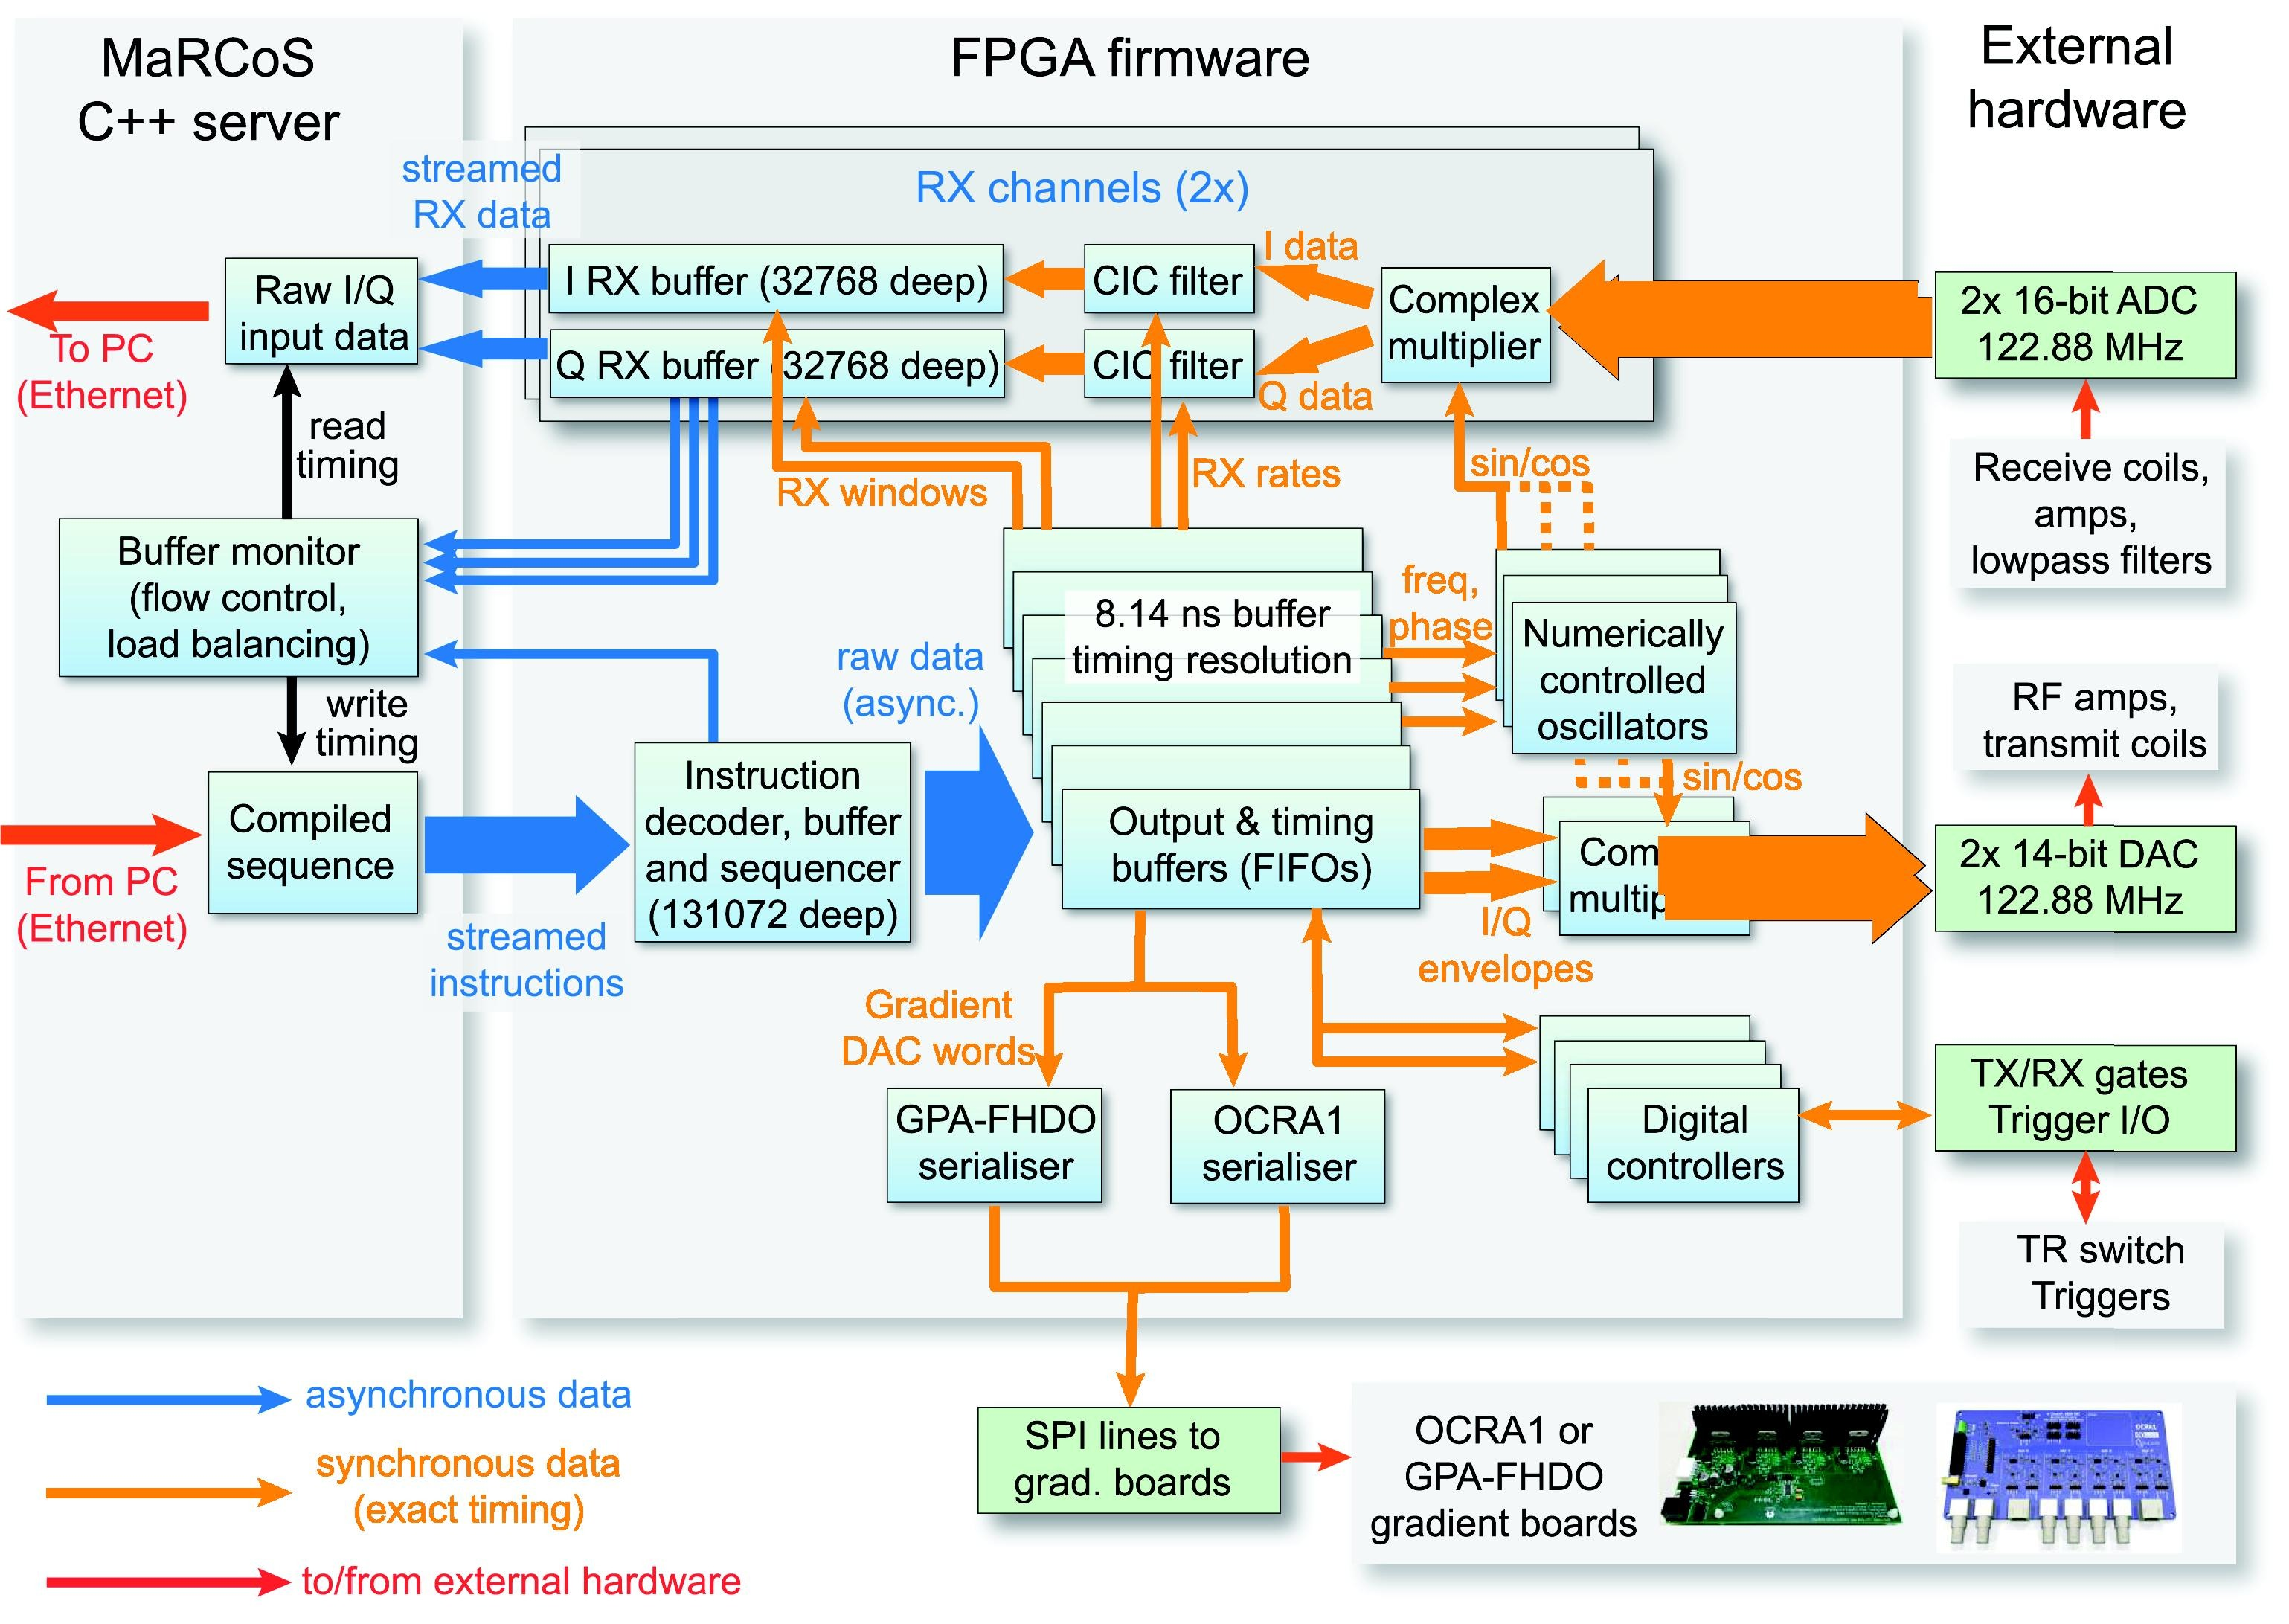
\includegraphics{images/marcos.jpg}
    \caption{\captiontitle{MaRCoS system architecture.} \enquote{The server receives a sequence from the client PC via Ethernet and streams it to the FPGA firmware, where it is translated into time-synchronous hardware operations including RF and gradient outputs. The firmware receives data from the ADCs, demodulates and filters it, and saves it into RX buffers, from which it is read by the server and sent to the PC} \cite{negnevitskyMaRCoSOpensourceElectronic2023}, Figure 3}
    \labfig{marcos}
\end{figure}

\section{The power amplifier}
\begin{marginfigure}[-4.5\baselineskip]
    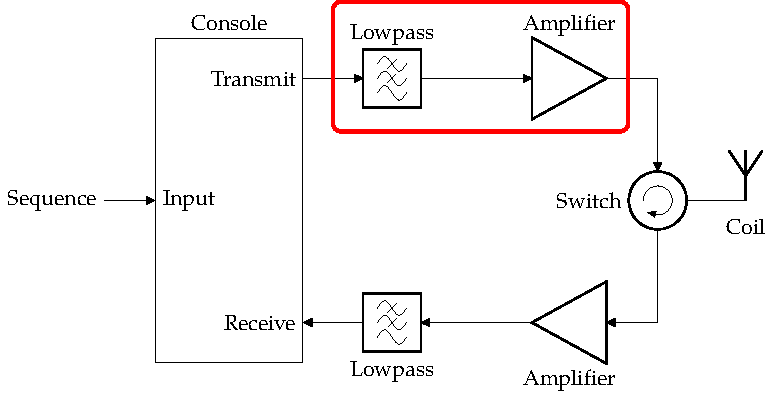
\includegraphics{block_diagram_highlight_tx.pdf}
    \labfig{block-diagram-pa}
\end{marginfigure}

Building of the power amplifier
\begin{figure}[hbt]
    \centering
    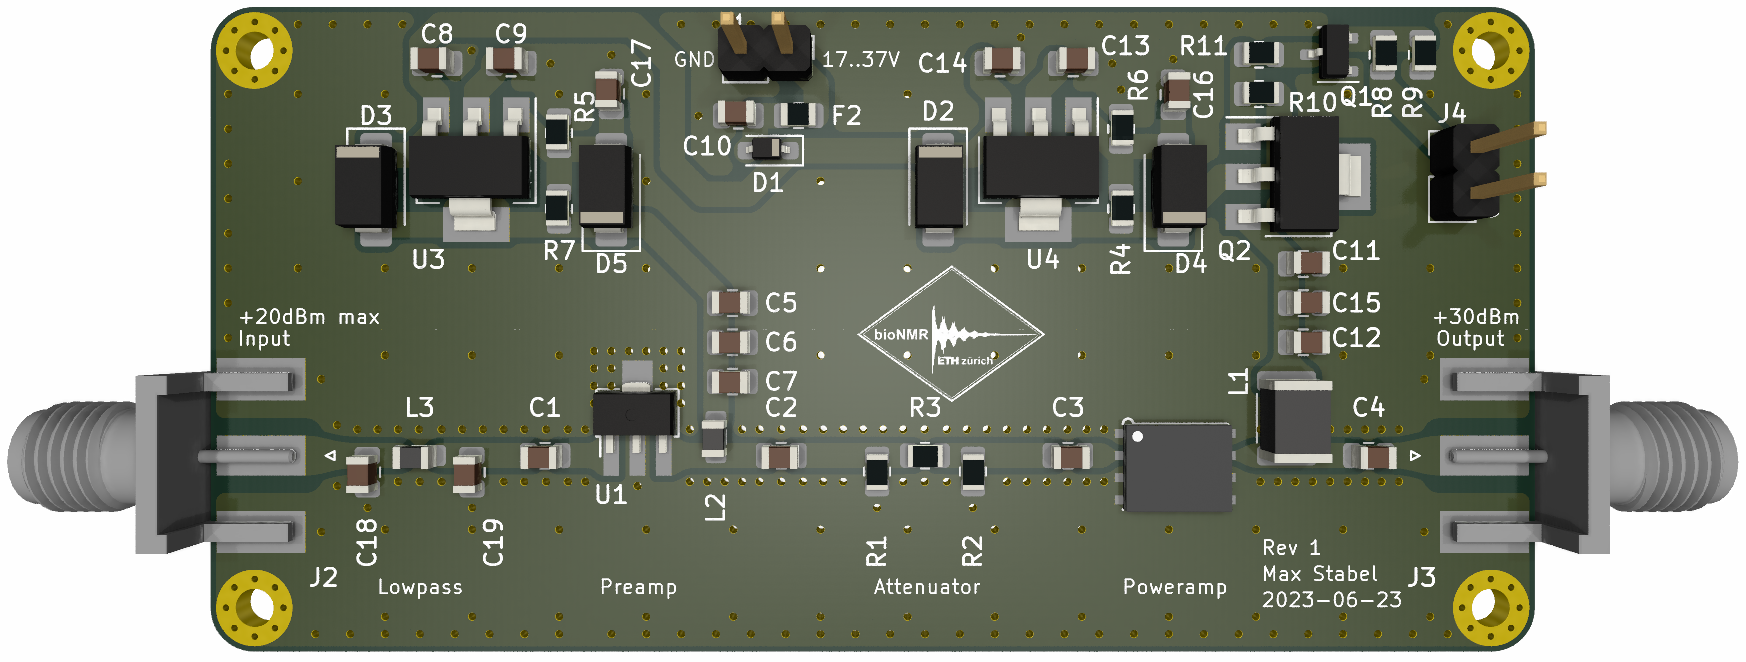
\includegraphics{images/poweramp.png}
    \caption{\captiontitle{\acrshort{rf} power amplifier.} 3D rendering of the power amplifier \acrshort{pcb} in KiCAD. The signal travels from left to right with the power supply circuitry above. It contains two \acrshort{mmic} amplifier stages, the AD5536 and the PHA-202+. A \qty{-6}{\deci\bel} attenuator was added in between and a passive low-pass filter in front (\(f_c = \qty{35}{\mega\hertz}\)). \(G \approx \qty{32}{\deci\bel}\), \(P_{\qty{1}{\deci\bel}} \approx \qty{+30}{\deci\belm}\)}
    \labfig{poweramp}
\end{figure}

\section{The switch}
\begin{marginfigure}[-4.5\baselineskip]
    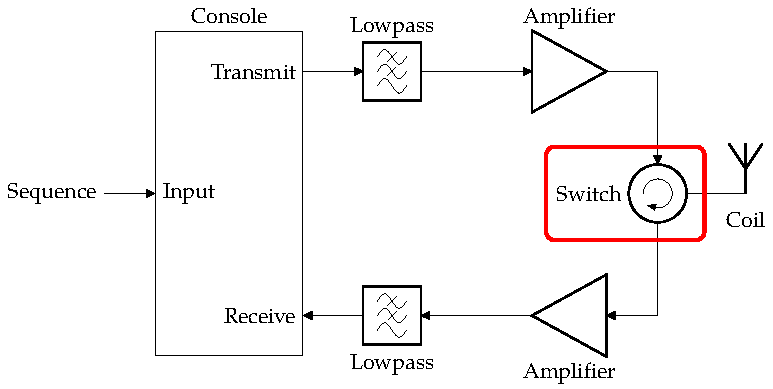
\includegraphics{block_diagram_highlight_switch.pdf}
    \labfig{block-diagram-switch}
\end{marginfigure}
building of the switch

\begin{figure}[hbt]
    \centering
    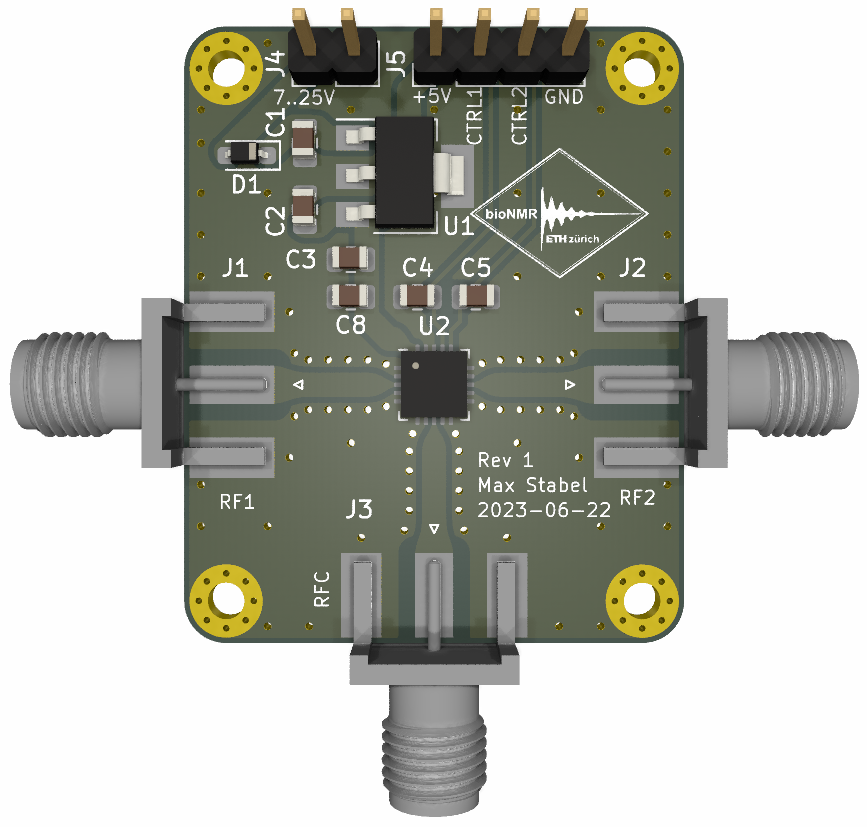
\includegraphics{images/tr_switch.png}
    \caption{\captiontitle{\acrshort{rf} \acrshort{tr} switch} 3D rendering of the switch \acrshort{pcb} in KiCAD. The transmit and receive amplifiers are connected on the left and right, the probe at the bottom connector. The central part is a Qorvo QPC6324 \acrfull{spdt} switch. Above it is a linear power supply and connection pins for active switching and power supply.}
    \labfig{switch}
\end{figure}


\section{The probe}
\begin{marginfigure}[-4.5\baselineskip]
    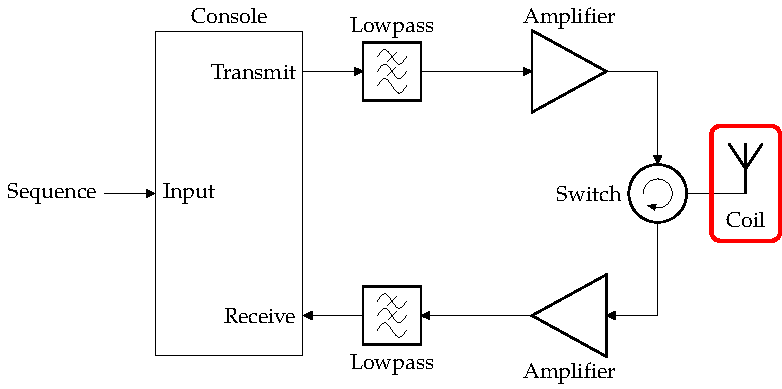
\includegraphics{block_diagram_highlight_coil.pdf}
    \labfig{block-diagram-coil}
\end{marginfigure}
building the coil

\begin{figure}[hbt]
    \centering
    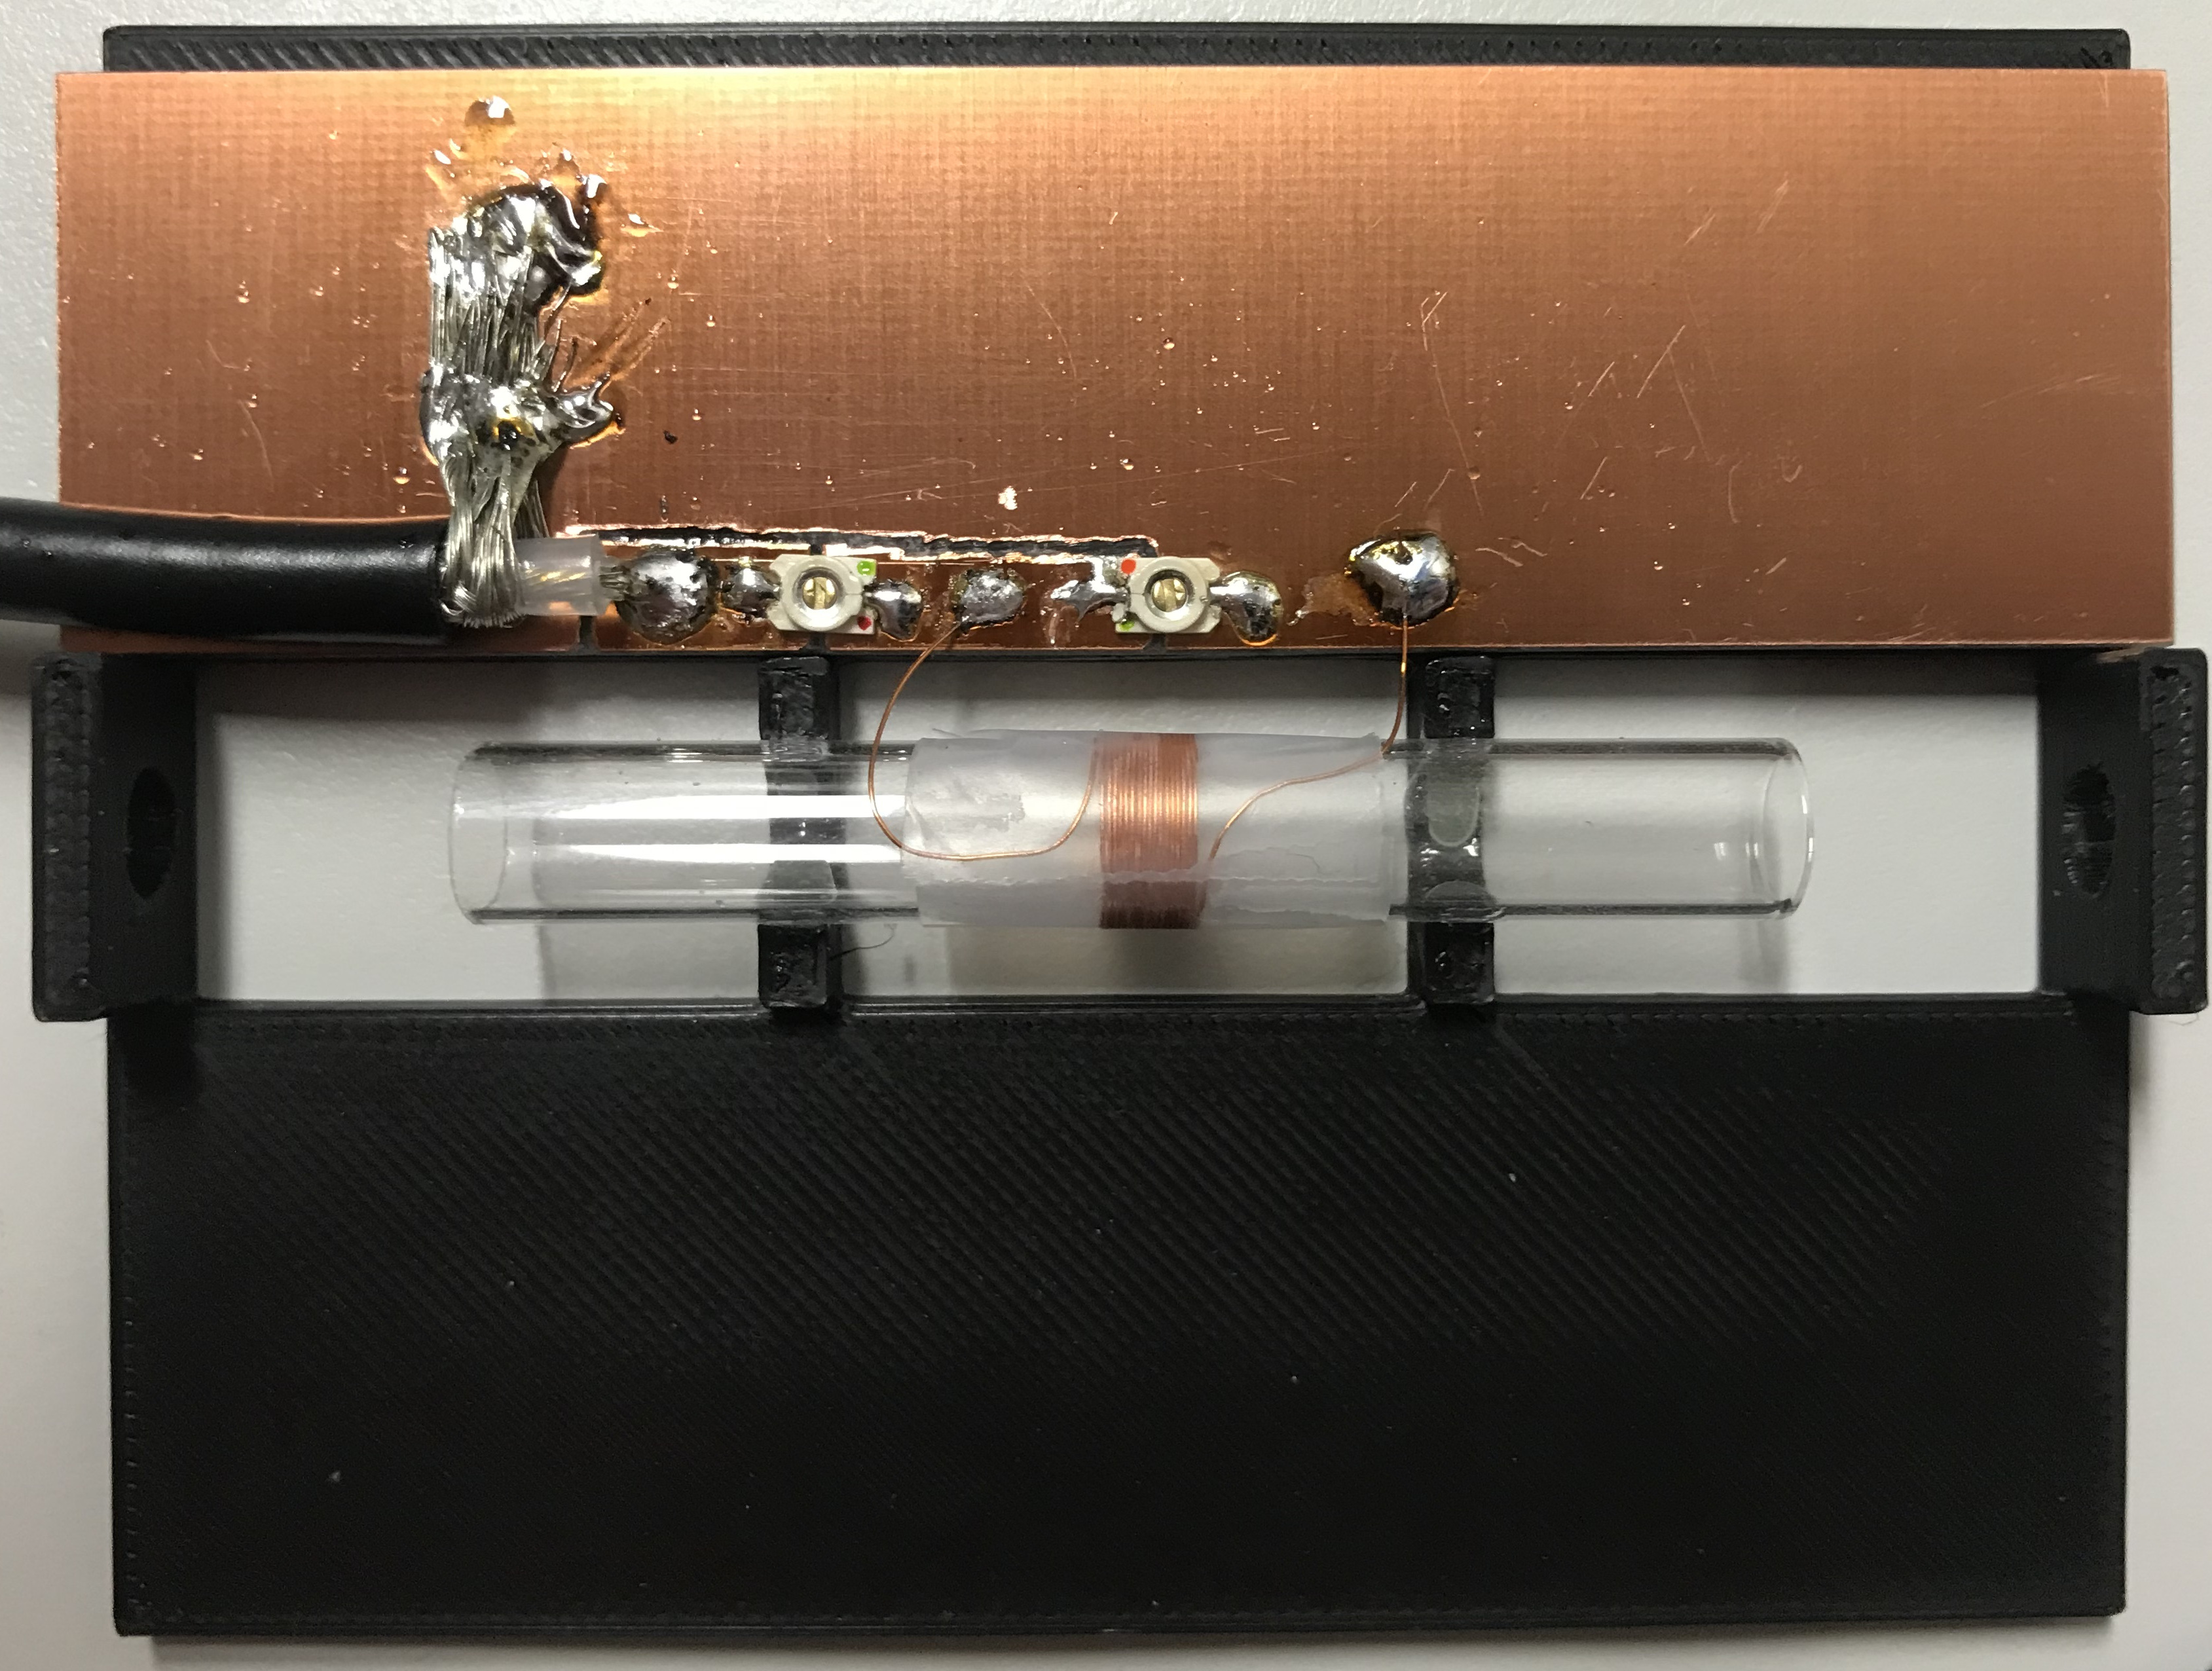
\includegraphics{images/probe.jpg}
    \caption{\captiontitle{Probe holder and \acrshort{rf} coil with tuning and matching capacitors} The capacitors are tunable from \qtyrange{4.5}{20}{\pico\farad} of make JZ200HV. The coil has a diameter of \(d = \qty{7.5}{\milli\meter}\), wire diameter \(D = \qty{0.2}{\milli\meter}\) and \(n = \qty{18}{turns}\) on a length of \(l = \qty{4}{\milli\meter}\). It has a measured inductance of \(L_{\qty{1}{\mega\hertz}} = \qty{2.7}{\micro\henry}\) and a resistance of \(R_{\qty{1}{\mega\hertz}} = \qty{0.63}{\ohm}\). The body was 3D printed and the circuit cut by hand.}
    \labfig{switch}
\end{figure}

\section{The 32-channel current supply}
building the power supply

\section{The software}
\labsec{software}

design and development of the control software
short description of marcos

% Probably integrate above
\chapter{Building process}
\labch{building-process}

\chapter{Lessons learned}
\labch{lessons-learned}